\section{Experimental Evaluation}
\label{sec:eval}

The evaluation asks whether one governed supervisory path can be exercised,
inspected, and repeated across heterogeneous industrial jobs, not whether one
optimizer beats another. Four questions organize the evidence: protocol closure
and governance attribution (Q1), the AgentTeam workflow (the lead--worker team
runtime of Fig.~\ref{fig:runtime}) on one node and on a
multi-node line (Q2), the deterministic cast-film loop (Q3), and attainment for
four process missions (Q4), each instantiating the path of
Fig.~\ref{fig:walkthrough}. Q1--Q4 map onto the contributions just
listed---Q1 exercises the integration boundary and attributes the governance
mechanism, while Q2--Q4 occupy the strategy slot from scripted policies to
concurrent missions.

\subsection{Testbed, Evidence Snapshot, and Scope}
\label{sec:testbed}
The snapshot is integrated run \resRun{} (seed \resSeed, commit \resCommit,
harness \resHarness, completed \resEvidenceDate), archived with raw reports and
mission logs; ablation companion \resAblationRun. Scripted external
policies call the
governed tools under a deployed member identity; two live agent-engine turns
check that the same slot accepts an engine
(archived trace headers record the harness, provider, and model:
omp, glm-5.3-flash). The
standing single-node preset is a cast-film extrusion line tuned through the
die-head heater setpoint (objective $J$ is the blueprint's weighted score over
thickness conformance, defect rate, energy, and throughput under
melt-temperature and pressure constraints---larger is better); each scenario
contributes one trajectory from
its seed-42 initial state.

\subsection{Test Procedure and System-Level Profile}
\label{sec:procedure}
The procedure is a \resPhases-phase integrated suite scoring
\resChecksPass{}/\resChecksTotal{} checks with no warnings or failures---an
author-defined regression summary, not an external certification---probing one
claim per phase, from preset loading against the offline optimum
($J^{*}=\resJstar$) and per-protocol interception through the record, recipe,
approval, and parameter-layer drills to the controller benchmark, second
preset, backstop drill, and campaign (Section~\ref{sec:scenarios}).

Figure~\ref{fig:systemexec} reports where the time goes: Panel~(a) shows each
phase's wall time (log scale). Deterministic governance steps---admission,
binding checks, record writes, recipe lifecycle---complete in milliseconds to
seconds, so the platform's per-intervention cost is validation logic; the long
tail sits in the replaceable strategy slot (the live engine turns take
\resLlmWall{} and \resGoalWall) and the observation cadences (the backstop
drill spans \resBackstopDrill, firing at \resBackstop). Panel~(b) is the
transparency tier: the closed-loop objective after two writes, normalized by
$J^{*}$; all three seeds land within 3.5 percentage points of the oracle
(Section~\ref{sec:controller}).

\begin{figure}[!t]
\centering
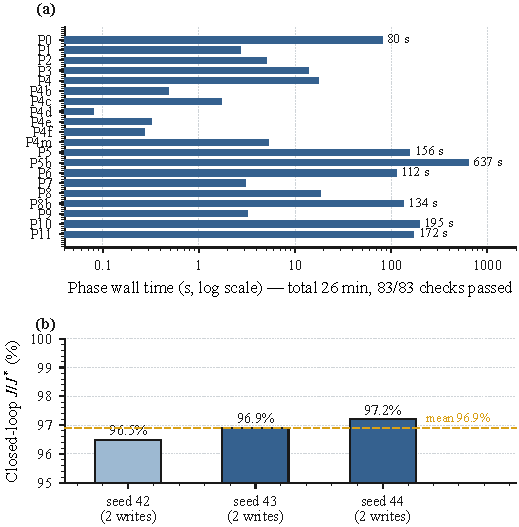
\includegraphics[width=\columnwidth]{resources/fig-system-evaluation.pdf}
\caption{Run \resRun at system level. (a)~Phase wall time (log scale); bar
labels are harness phase identifiers. (b)~Closed-loop objective $J$ after two
governed writes as a fraction of $J^{*}$, per seed, with no write rejected;
the annotated mean is 96.9\%.
Panel (a) is environment telemetry,
not a service-level bound.}
\label{fig:systemexec}
\end{figure}

\subsection{Q1: Protocol Closure and Governance Attribution}
\label{sec:protocol}
On the five protocol lines the suite stores \resDaqSamples{} DAQ samples through
real drivers, including a Modbus RTU-over-TCP satellite; governed writes are
accepted and read back on Modbus TCP, OPC~UA, MQTT, and HTTP (per-line medians
\resTcpP, \resOpcP, \resMqttP, and \resHttpP). Four of the five lines are
writable---the Modbus RTU-over-TCP satellite is acquisition-only in this
deployment. Because one
admission, record, and verdict path
serves every request, the residual spread is consistent with transport
differences. Each writable line rejects 6/6 configured
out-of-window probes while accepting its legal write, so all 24 probes are
intercepted; a dedicated window-interlock drill (the Stage-1 gate of
Fig.~\ref{fig:runtime}) adds decision-boundary probes at the
window edge and just outside it, and exercises both admission branches, line
running and line stopped---the interlock discriminates rather than merely
blocks.

Two drills then separate truth paths that one success flag would collapse:
a frozen-measurement drill accepts a write and a consistent readback while the
measurement stays out of window, and the backstop records a system-judged
rollback \resBackstop{} later---readback closes the command path, the backstop
closes the record, and neither is a settling time. A second preset with
different signals and dynamics is then commissioned by configuration
alone (zero framework code changes); across both presets, 33 configured probes
are rejected on seven writable lines---six per line on the first, three per
line on the second---the same admission code discriminating on
signal maps it had not previously exercised.

The parameter layer passes \resParamChecks{} checks and makes the interval
geometry of Section~\ref{sec:objective} observable: a four-layer chain (node
$[50,200]$\,rpm, parameter
$[143.7,156.3]$\,rpm, product $[146.22,153.78]$\,rpm, recipe
$[141,159]$\,rpm) narrowing to one admitted interval, each rejection
attributable to its excluding layer. A manual binding instead suspends a
request visibly and unblocks it on approval, after which the
write takes effect at the device (automated round-trip latency \resHitlLatency):
workflow mediation, not physics.

\begin{table}[!t]
\centering
\caption{Governance ablation on companion run \resAblationRun{} (three deterministic repetitions with identical counts; 18 probes per arm: 12 hard-range and 6 window-class).}
\label{tab:ablation}
\footnotesize
\setlength{\tabcolsep}{3.2pt}
\begin{tabular}{@{}lrrr@{}}
\toprule
Arm & Rejected & Executed breaches & False blocks \\
\midrule
Full governance & \resFullIntercept & 0 & 0 \\
No window interlock & \resNoInterlockIntercept & 6 & 0 \\
No readback check & \resNoReadbackIntercept & 0 & 0 \\
Both relaxed & \resUngatedIntercept & 6 & 0 \\
\bottomrule
\end{tabular}
\end{table}

Table~\ref{tab:ablation} attributes the rejection rather than assuming it, on a standalone admission-pipeline fixture kept outside the scenario simulators; counts are identical across the three deterministic repetitions, and the per-request latencies archived for every arm overlap at this resolution---we claim only that no overhead is visible on this fixture. Full governance and the no-readback arm reject 18/18 probes, whereas removing the window interlock, alone or with the readback check, lets the six window-class probes execute and be journaled. Two readings follow. First, prevention is the
window interlock's job: the readback check contributes nothing to interception---it
closes the command path after execution---yet is retained because it makes a
written-but-unconfirmed command visible. Second, attribution
survives removal: the six executed breaches still appear in the journal, so a
relaxed configuration degrades from prevention to detection. The hard range is
structurally unbypassable and the soft window is
its removable part; no arm records a false block.

\subsection{Q2: The AgentTeam Optimization Workflow and Its Results}
\label{sec:agentteam}
The workflow ran end to end on the cast-film line and then on a larger BOPET line
(Section~\ref{sec:tasklifecycle}); a scripted policy rather than a language model
issued the writes in both missions (the two live engine turns follow at the
end of this subsection). On the single-node mission one write sufficed: the
die-head heater setpoint moved from \resMissionFrom{} to
\resMissionTo{}\,$^{\circ}$C and the observation
settled at \resMissionPv{}\,$^{\circ}$C against
\resMissionTarget\,$^{\circ}$C, the journal attributing the change to the
agent identity, the task closing \texttt{COMPLETED}.

The BOPET mission is the multi-node case: nine devices and 49 signals
(\resBiaxSp{} writable, \resBiaxDaq{} readable), all created by the
\emph{ensure} pass, whose driver tests passed on all nine endpoints. Thickness
started at \resBiaxStart\,$\mu$m against
$\resBiaxTarget\pm\resBiaxTol$\,$\mu$m. Three governed writes on three distinct
nodes---casting speed $32\!\rightarrow\!33.8$\,m/min, fast-roll speed
$118\!\rightarrow\!120.3$\,m/min, and rail width $3000\!\rightarrow\!3035$\,mm---brought it to
\resBiaxFinal\,$\mu$m. Each write opened a record, received \texttt{keep}, and
left an agent-attributed journal entry, while melt temperature stayed near
291\,$^{\circ}$C and the parent task reached \texttt{COMPLETED}. In both
missions the governed-write count matched the number of accepted setpoint
changes---by construction, since each write traverses the same admission,
record, and verdict steps regardless of line size.

In the bounded turn the agent read the node's semantic card, sampled a baseline
through \texttt{daq\_query}, wrote $197.48\,^{\circ}$C, waited,
resampled, and closed the record with \texttt{keep}, finishing in
\resLlmWall{} and storing one lesson: the acquisition-limit flag can lag the
live value. The goal-driven turn took \resGoalWall: it queried the journal
and its own memory, found neither, measured 53.79\,$\mu$m at 150\,rpm
against a self-selected target of $52.0\pm0.8$\,$\mu$m (the governed path, not
a predicate, constrains this turn), inferred from mass conservation
($h\propto N/v$) that
screw speed should fall by about 5\,rpm, applied the change in steps, judged
each write on measured evidence, refined its gain estimate from 0.22 to
0.36\,$\mu$m per rpm, and settled thickness at \resGoalFinal\,$\mu$m; it also
saved the recipe---authorship attributed and audit-logged, activation
role-gated.

\subsection{Q3: The Deterministic Closed Loop}
\label{sec:controller}
Seeds 42--44 each issue two governed writes with no rejection, raising the
cast-film objective $J$ (larger is better) from $J_{0}\approx\resJzero$ to
$J/J^{*}=\resControllerMin$, \resControllerMean, and \resControllerMax{} on
the three seeds, against the simulator's offline reference
$J^{*}=\resJstar$ obtained by
exhaustive grid search over its steady-state map. The residual gap to
unity is expected: $J^{*}$ is an oracle with full model
knowledge, which an online policy seeing only process observations cannot in
general match. What the benchmark establishes is narrower: the governed path
passes a conventional controller's writes through unmodified---admissible,
journaled, and read back---and no ungoverned performance arm was run, so the
path's
transparency is shown for admission and evidence handling rather than measured
as a performance delta.

\subsection{Q4: Four Process Missions}
\label{sec:scenarios}
The campaign runs four lines concurrently, each provisioned from a blueprint
by the \emph{ensure} pass and given one channel; all four attain their archived
predicates, evaluated from subsequent observations, not the task
state. The controlled quantity moved from
\resInjStart{} to \resInjFinal\,g, \resWwtpStart{} to \resWwtpFinal\,mg/L,
\resAnnealStart{} to \resAnnealFinal\,HV, and \resBiaxStart{} to \resBiaxFinal\,$\mu$m;
mission clocks (\resInjWall, \resWwtpWall, \resAnnealWall; the BOPET clock was
not retained) are simulator wall time under accelerated dynamics, not physical
durations.
Figure~\ref{fig:multiscenarioopt} archives the trajectories: the curve is the
observed controlled variable, the hatched band its window, and the filled
terminal marker the predicate-satisfying observation; each mission iterates
the same loop---read, write inside the admitted interval, observe, judge---so
one governed loop produces all four trajectories.

\begin{figure*}[!t]
\centering
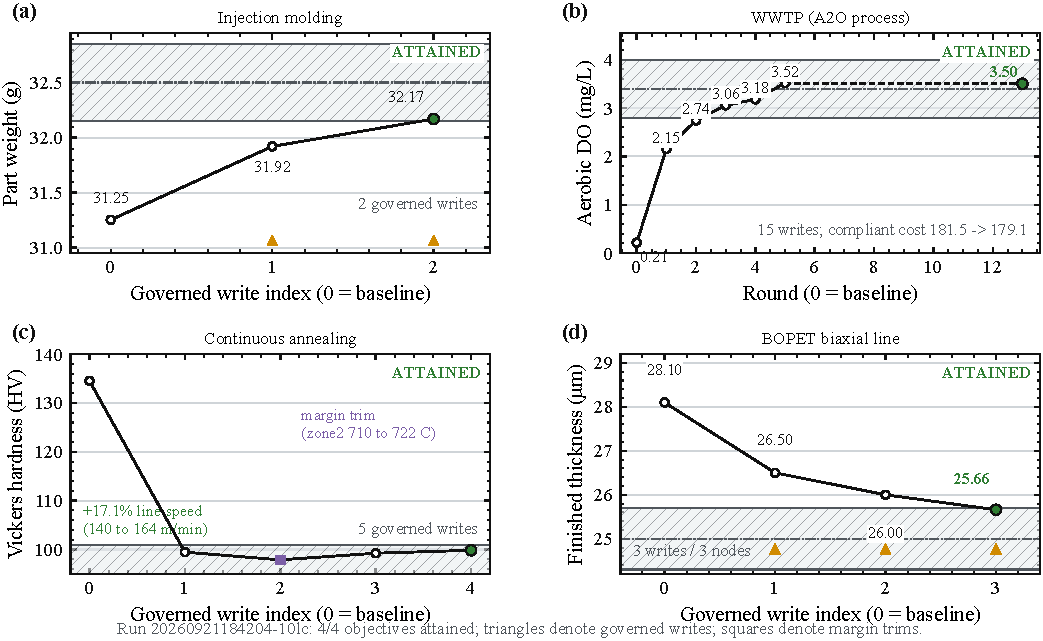
\includegraphics[width=0.78\textwidth]{resources/fig-multiscenario-optimization.pdf}
\caption{Archived trajectories of the four missions in run \resRun. Hatched
bands are objective windows, the dash-dotted line the target, filled terminal
markers the predicate-satisfying observations. Panel (a)
marks governed-write rounds with triangles, Panels (c) and (d) index points by
governed write, and Panel (b) tracks dissolved oxygen through the mission's
stages (its round axis includes the 15 governed writes) with write count and
cost index annotated; the square in (c) marks the zone-2 margin trim. All four terminal markers lie inside
their objective window. Curves are simulator observations under scripted
policies, not physical measurements.}
\label{fig:multiscenarioopt}
\end{figure*}

Panel~(a): injection molding is the minimal case---two writes raise the hold pressure
from 45 to 58.2\,bar and the hold time
from 6 to 10.64\,s, and the policy stops at
\resInjFinal\,g inside $32.5\pm0.35$\,g in \resInjWall, with the flash and sink
guards inside their limits.

Panel~(b): wastewater treatment, the longest mission, has two stages.
Aeration, caustic, and coagulant dosing bring dissolved oxygen from
\resWwtpStart{} into $3.4\pm0.6$\,mg/L under the effluent guards on
COD, ammonia, total phosphorus, pH, and turbidity; the policy then lowers blower
frequency and caustic dose, ending after \resWwtpWrites{} writes at
\resWwtpFinal\,mg/L in \resWwtpWall{} with the simulator-internal
compliance-cost index (Fig.~\ref{fig:multiscenarioopt}b), the scenario's
operating-cost proxy, down from
\resWwtpCostStart{} to \resWwtpCostFinal. Two blower
steps are the most informative events: both writes were
admissible and journaled, the post-write observation lost compliance margin, and
the verdict stage reverted them---rejection of a bad proposal lives in the
evidence, not in the admission gate.

Panel~(c): annealing starts far outside the hardness window (\resAnnealStart\,HV
at 140\,m/min). Raising zone-3 temperature to 850\,$^{\circ}$C brings hardness to
99.46\,HV; one zone-2 trim and two line-speed steps then hold $95\pm6$\,HV while
raising line speed by \resAnnealGain, and a further attempt at
\resAnnealSpeedTried\,m/min is reverted for leaving the margin. All
\resAnnealWrites{} governed writes are journaled; the panel's baseline-indexed
axis plots the states they produced---the fifth (the reverted
\resAnnealSpeedTried\,m/min attempt) returned the process to the prior state,
so it shares that position and is distinguished only in the journal. The guard
is multi-objective---hardness and throughput must hold
together---and the predicate holds in \resAnnealWall{} only because the
margin-violating speed was undone, on record.

Panel~(d): BOPET is the nine-device mission of Section~\ref{sec:agentteam}
executed under the campaign harness, moving thickness from \resBiaxStart{} to
\resBiaxFinal\,$\mu$m inside $25.0\pm0.7$\,$\mu$m. In this mission completion
and the predicate agree, yet they remain separate records, so a later missed
objective would still be visible.

\subsection{Cross-Scenario Reading}
\label{sec:synthesis}
Read together, the four missions bound what the framework contributes:
platform-side behavior is invariant while the write economy---the
governed-write count each scripted policy needs---varies by more
than a factor of seven (2, 15, 5, and 3 writes) and the mission clock by more
than six (26.48\,s to 169.27\,s over the three retained clocks), both produced
by construction in the scenario-specific slot. The three reversions (two
blower steps, one speed step) show caller-side verdicts doing real work; that
all four terminal markers lie inside their bands is an observed outcome, not a
structural property. Margins are narrow but on record: 32.17\,g sits 0.02\,g
above 32.15\,g, 100.08\,HV 0.92\,HV below 101\,HV, and
25.66\,$\mu$m 0.04\,$\mu$m below 25.7\,$\mu$m; the compliance-cost index
ends 1.3\% lower.
